Our method takes as input, a profile view face, $A_p$, and an exemplar database, $D$, consisting of
wide range of profile, frontal pose pairs for different persons. We then proceed to frontalize
the face in two steps. First, we run facial landmark
detection~\cite{kazemi2014one} on the input face, and using it we retrieve the most similarly posed face 
$I^i_p$ and its corresponding frontal view face $I^i_f$, from
database $D$. When profile views of two faces match, there is high likelihood that the two persons
have similar facial structures. We exploit this property to get geometrical transformations required
for frontalization of the input face.
% Simultaneously, using the landmarks on the face, we define a set of corresponding planes 
% in {\sc 3d} for all of $A_s$, $B_s$ and $B_f$. 
Simply put, we obtain the frontal view of $A_p$ by using the affine transformations between $A_p$
and $I_f$. One recently proposed state-of-the-art method~\cite{DBLP:journals/corr/HassnerHPE14} uses a generic {\sc 3d}
model for computing this transformation. This leads to loss of important discriminate structural information
unique to an individual. Since we are finding a nearest profile exemplar and its corresponding
frontal view face, structural information is still preserved for an individual face in our case.
                 
\begin{figure*}
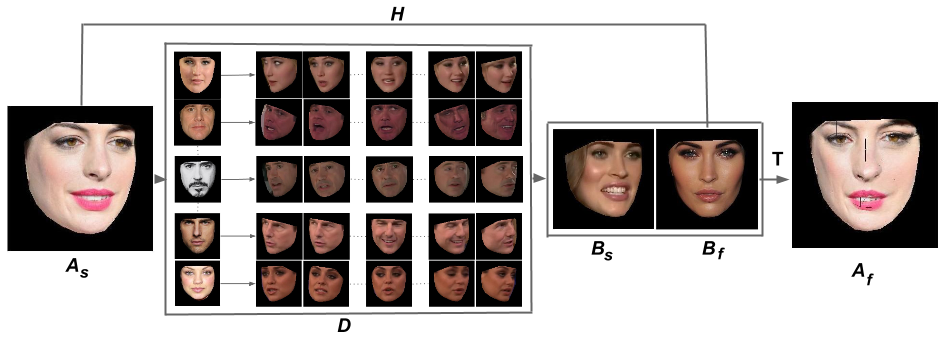
\includegraphics[width =16cm,height=6.6cm]{front/figures/Method_Pipeline.png}
\caption{Figure shows the generic pipeline used in our approach. Given the input image (left most
block) we use the exemplar database (second block) to compute the nearest profile view (third block,
first image). We then use the correspondences between the profile and frontal views of the
selected exemplar pair (third block) to compute the affine transformation $H$ between the input
image and the frontal exemplar, and use it to produce the \emph{frontalized output} (right most block).}
\label{fig:method_pipeline}
\end{figure*}

Let $P = (X, Y)$, denote the landmark locations on the face, where $X=(x_1, x_2, .. , x_{68})$ and
$Y=(y_1, y_2, .. , y_{68})$ are vectors of $X$ and $Y$ coordinates respectively. We consider 68 landmarks 
which includes feature points such as eye corners, nose tip, mouth line and jaw line. 
We use the dlib~\cite{kazemi2014one} implementation for landmark localization.  Note that landmarks of images in $D$ have been pre-computed.
We also manually predefine 110 planes for a face using these landmarks. For example, the ends of two
eyebrows and the beginning of the nose form a plane (see Figure~\ref{fig:triangulation}). This has to be done
only once since these planes connect the same fiducial points irrespective of the face. Each plane is
defined by 3 landmark locations. 

Let $T = \{t_{1}, t_{2}, \ldots , t_{110}\}$
represent the set of planes defined in {\sc 3d} for a face image. Given planes of one
profile-frontal image pair $T_p^m \& T_f^m$, in D, we define $H^{m} = \{H_1^m, H_2^m, \ldots ,
H_{110}^m\}$ as the affine transformations between corresponding planes, computed using point correspondences from the facial landmarks. That is, 
\begin{equation}
  t_{f}^{m,i} = t_{p}^{m,i} \times H_i^m \label{eq:affine_transfomraiton}
\end{equation} 
where the subscript $p$ denotes profile, and the subscript $f$ denotes frontal views.

Given the landmarks $P$ for images in the database $D$, we now
proceed to frontalize using the following steps.
